\documentclass[]{aiaa-tc}

\usepackage{authblk}
%\usepackage[margin=3cm]{geometry}

\title{Coupled Aero­-Structural-Propulsive­ Design of an Ultra­Light, Highly Flexible Aircraft}

\author[1]{Justin Gray}
\author[1]{Jeffrey Chin}
\author[2]{Kevin Reynolds}
\author[3]{Dr. Graeme Kennedy}
\author[4]{Dr. Juan Alonso}
\author[4]{Dr. Todd Reichert}

\affil[1]{Aerospace Engineer, NASA Glenn Research Center - LTA Branch}
\affil[2]{Aerospace Engineer, NASA Ames Research Center - TI Branch}
\affil[3]{Assistant Professor, Georgia Institute of Technology, School of Aerospace Engineering}
\affil[4]{Associate Professor, Stanford University, Department of Aeronautics and Astronautics}
\affil[5]{Vice President of Aerodynamics, AeroVelo Inc.}

\begin{document}

  %\maketitle

  \vspace{4em}
  \begin{center}
    A proposal to the NASA ARMD Team Seedling Program: 
    \vspace{2em}

    {\Huge Coupled Aero­-Structural-Propulsive­ Design of an Ultra­Light, Highly Flexible, Human Powered Aircraft}

    \vspace{2em}
    submitted to the NASA Aeronautics Research Institute by: 

    \vspace{3em}
    [Insert Lots of Logos/Picture Here]
    \vspace{3em}


  \end{center}


  \begin{tabular}{l l}
    Principal Investigator & Justin S. Gray; NASA Glenn Research Center, Propulsion Systems Analysis Branch \\ 
    & \\
    Co-Investigators & Dr. Juan Alonso; Stanford University, Department of Aeronautics and Astronautics \\
                     & Dr. Graeme Kennedy; Georgia Institute of Technology, School of Aerospace Engineering \\ 
                     & Dr. Todd Reichert; Vice President of Aerodynamics, AeroVelo Inc. \\
    & \\ 
    Team Members & Cameron Robertson; Vice President of Structures, AeroVelo Inc. \\ 
                 & Jeffrey Chin; NASA Glenn Research Center, Propulsion Systems Analysis Branch \\
                 & Kevin Reynolds; NASA Ames Research Center, ??? Branch \\
  \end{tabular}

  \newpage

  \section{Introduction}

    The Fundamental Aeronautics Program has identified \textbf{Ultra Efficient Commercial Vehicles} as 
    a key research thrust. A number of concepts have been proposed along those lines, such as 
    the MIT D8 double­-bubble and the Boeing SUGAR­-High truss­-braced wing. These aircraft rely on 
    very high­-aspect ratio, extremely flexible wings to help achieve very low energy consumption. 
    Long endurance solar sensorcraft, being proposed by companies such as General Atomics and 
    Scaled Composites, share a similar approach to minimizing energy consumption by leveraging highly 
    flexible wings. This begs the question, \textbf{``How does aircraft design change to take full 
    advantage of highly flexible structures?''} The Vision 2030 CFD study also highlights the 
    design of highly flexible wings as a modeling grand challenge problem. That study specifically 
    highlights the need for highly multidisciplinary, tightly coupled design process with high 
    fidelity tools to address this grand challenge.

    Aircraft empty weight reduction is a major driving factor pushing designs toward highly flexible structures. 
    While lower weight helps to achieve lower energy consumption, the flexibility in the structures also 
    generates very large deflections and highly non-linear structural responses. These characteristics mean that 
    structural failure is a major design consideration.[CITATION HERE] Thus it is interesting to consider the question, 
    \textbf{``How can structural health monitoring technologies be used to enable lighter 
    weight structures?''}, to address the \textbf{Real­-Time System­-Wide Safety Assurance} thrust. 

    One of the major challenges associated with designing highly flexible wings is that the as-flow configuration 
    is dramatically different than the as-built configuration (jig shape). With modern aeroelastic techniques, 
    we can now design more conventional wings taking this into account[CITATIONS NEEDED]. However, highly flexible
    structures bring new challenges that need to be addressed. Besides the non-linear structural 
    response these wings also tend to have different load distributions from conventional wings. Many of the concepts 
    also include a distributed propulsion aspect, with propellers spread out across the wing. The affect of the 
    propulsion system not only on the structures, but also on aerodynamics and the overall controllability 
    of the aircraft need to be considered. These aspects push the 
    limits of todays most advanced high-fidelity aeroelastic design techniques, which currently rely on linear structural 
    models and don't account for any propulsion interactions. 

    AeroVelo Inc. has invited NASA to participate in the design and flight testing of a new, highly flexible aircraft. 
    Collaborating with AeroVelo will allow us to develop and validate the necessary tools and methods for a 
    next-generation aircraft design tool. Aero Velo, the team that won the Sikorski Human Powered Helicopter Prize in 2013, 
    is planning to build a human powered aircraft to achieve the Kremer Marathon Challenge; fly a human 
    powered aircraft 26.1 miles in under 1 hour. Human powered aircraft share many of the same key qualities 
    with other highly flexible aircraft. Since the only available power is that of the human pilots, minimizing 
    energy consumption is of paramount concern. As such, they invariably possess ultralight highly flexible wings. 
    A recent human powered aircraft, the Musculair II, employed an advanced all-composite wing structure 
    with a stressed skin design[CITATION NEEDED]. The initial concept for AeroVelo's Marathon aircraft includes 
    a span loaded structure with multiple pilots and multiple propellers distributed across the wing. These qualities 
    make human powered aircraft an excellent lower cost, low risk test bed for developing advanced design methods 
    for highly flexible structures. [Cool Picture Needed]

    In phase one of this effort, the analysis tools and coupled design environment will be built and 
    the detailed design marathon aircraft will be completed. In addition, sub-scale testing will be 
    performed to validate the individual aerodynamics and structural models. In phase two of the effort
    the aircraft will be built, tested, and flown to attempt the Kremer Marathon Challenge. Throughout 
    the effort, data will be collected to validate the analysis tools. At the completion of the effort 
    all the data collected, all of the models, and the final detailed design will be released under 
    an open-source license.

  \section{Objectives and Technical Approach}

    The overall objective of this work is to design, test, and fly a human powered aircraft, 
    capable of flying 26.1 miles in under 1 hour using state-of-the-art multidisciplinary 
    design optimization techniques. The design will be performed with fully coupled
    aerodynamic, non-linear structural, and propeller models. Working in the context of 
    a full aircraft design process, from conceptual all the way to detailed design, 
    provides a unique opportunity to apply multidisciplinary optimization methods and validate
    the results within a single project. 

    Phase one of the work will focus on the design of the aircraft. NASA Glenn Research Center, 
    NASA Ames Research Center, Stanford, and the Georgia Institute of Technology will be responsible 
    for collaboratively developing the propulsion, aerodynamic, and structural analysis 
    models needed as well as integrating them together for perform the coupled analysis. AeroVelo 
    use the models to perform the conceptual, preliminary, and detailed design of the actual marathon 
    aircraft in very close collaboration with the other partners. 

    \subsection{Model Integration (Glenn)}

    NASA Glenn's OpenMDAO Framework will serve as the integration tool for this effort. It's advanced 
    capabilities for code coupling with support for analytic gradients will be utilized to build 
    a design tool that integrates the high-fidelity models into a cohesive coupled design environment. 
    Engineers at NASA Glenn will be responsible for doing all the code integration into OpenMDAO. 

    \begin{figure}
        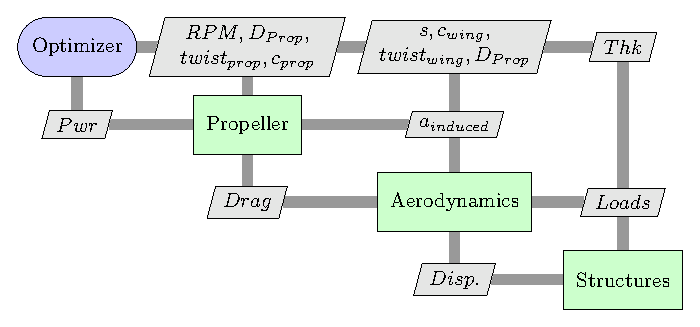
\includegraphics[width=\textwidt]{xdsm/overall}
    \end{figure}

    \begin{itemize}
        \item N2 diagram showing proposed data flow (Propeller, Wing, Structures, Mission)
        \item System level adjoint analytic gradients for large design spaces
        \item Geometry (GeoMACH, VSP, OpenCSM)
        \item Load and displacement transfer?? 
    \end{itemize}

    

    \subsection{Aerodynamic Modeling (Stanford / Ames)}

    Stanford's SU2 CFD tool, will be used for the aerodynamic analyses of both the wing and 
    the propellers. SU2 has been successfully applied to the design of propeller systems 
    and has support for actuator disk boundary conditions that will be needed to implement 
    the coupled wing­-propeller design process. It has been demonstrated to work in the low 
    Mach conditions that will be seen by this aircraft. It also provides adjoint derivatives 
    which are fundamental to the application of state­-of-­the-­art gradient based design 
    optimization methods. Researchers at Stanford will be responsible for building for developing 
    the aerodynamic models of the wing and will collaborate with NASA Glenn on developing the 
    propeller models. In addition they will provide support for integrating SU2 into the OpenMDAO 
    framework. 

    \subsubsection{Propeller Analysis (Ames)}
        \begin{itemize}
            \item SU2 can be applied using the rotating reference frame features for efficient high fidelity propeller design
            \item Lower fidelity tools may be even more efficient and could be highly accurate with good 2d airfoil data. Andrew Ning's 
            CCBlade is a good option. 
        \end{itemize}

    \subsubsection{Wing \& Fueselage Analysis (Stanford)}
        \begin{itemize}
            \item Laminar flow is a key design requirement for both the wing and the pilot farings. An inverse design approach can be employed 
            by specifying a desired pressure distribution. 
            \item TriPan is a lower fidelity option that also provides gradients and could possibly be employed to reduce computational cost. It might make sense to set things up so that SU2 and Tripan could be used interchangeably. 
        \end{itemize}

    \subsubsection{Wing-Propeller Coupling (Glenn/Stanford)}
        \begin{itemize}
            \item SU2 actuator disks for coupling
        \end{itemize}

    \subsection{Structural Analysis (GaTech)}

    The structural modeling will be performed with Toolkit for Analysis and of Composite 
    Structures (TACS). TACS has the necessary advanced capabilities such as adjoint derivatives 
    and efficient load and displacement transfer to enable coupled aero­-structural design. It also has 
    support for iso-geometric elements which will reduce the overall computational cost of the 
    structural analysis. Researchers at the Georgia Institute of Technology will be responsible for 
    building the structural models and providing support for integrating them into the OpenMDAO framework. 

    \subsection{Aircraft Design (AeroVelo)}

    AeroVelo will be responsible or the actual design and construction of the aircraft using the tools developed 
    by the other team members. They will also be responsible for building the structural test articles and designing 
    the structural validation tests. After the attempt has been made, NASA will be given access to 
    the aircraft to perform additional test flights to collect data. 

    \subsection{Wind Tunnel Testing}
        \begin{itemize}
            \item Expect airfoils to have a chord of about 2 feet. Flight speeds will be about 26 mph (40 feet/sec). Can we find a wind tunnel 
            that can test an article of that size at such slow speeds? 
            \item Another option would be to build a small test wing and fly it on a drone. Ames has the ability to rapidly prototype this kind 
            of drone and could provide actual flight tests. I suspect this would be a lower cost solution, but could 
            present measurement challenges. 
        \end{itemize}

    \subsection{Structural Testing}
        \begin{itemize}
            \item CFOSS system for structural tests?? 
            \item What kind of measurements are necessary to validate the codes? 
            \item What kind of measurements are necessary to validate the design? 
        \end{itemize}

    
    \begin{figure}
        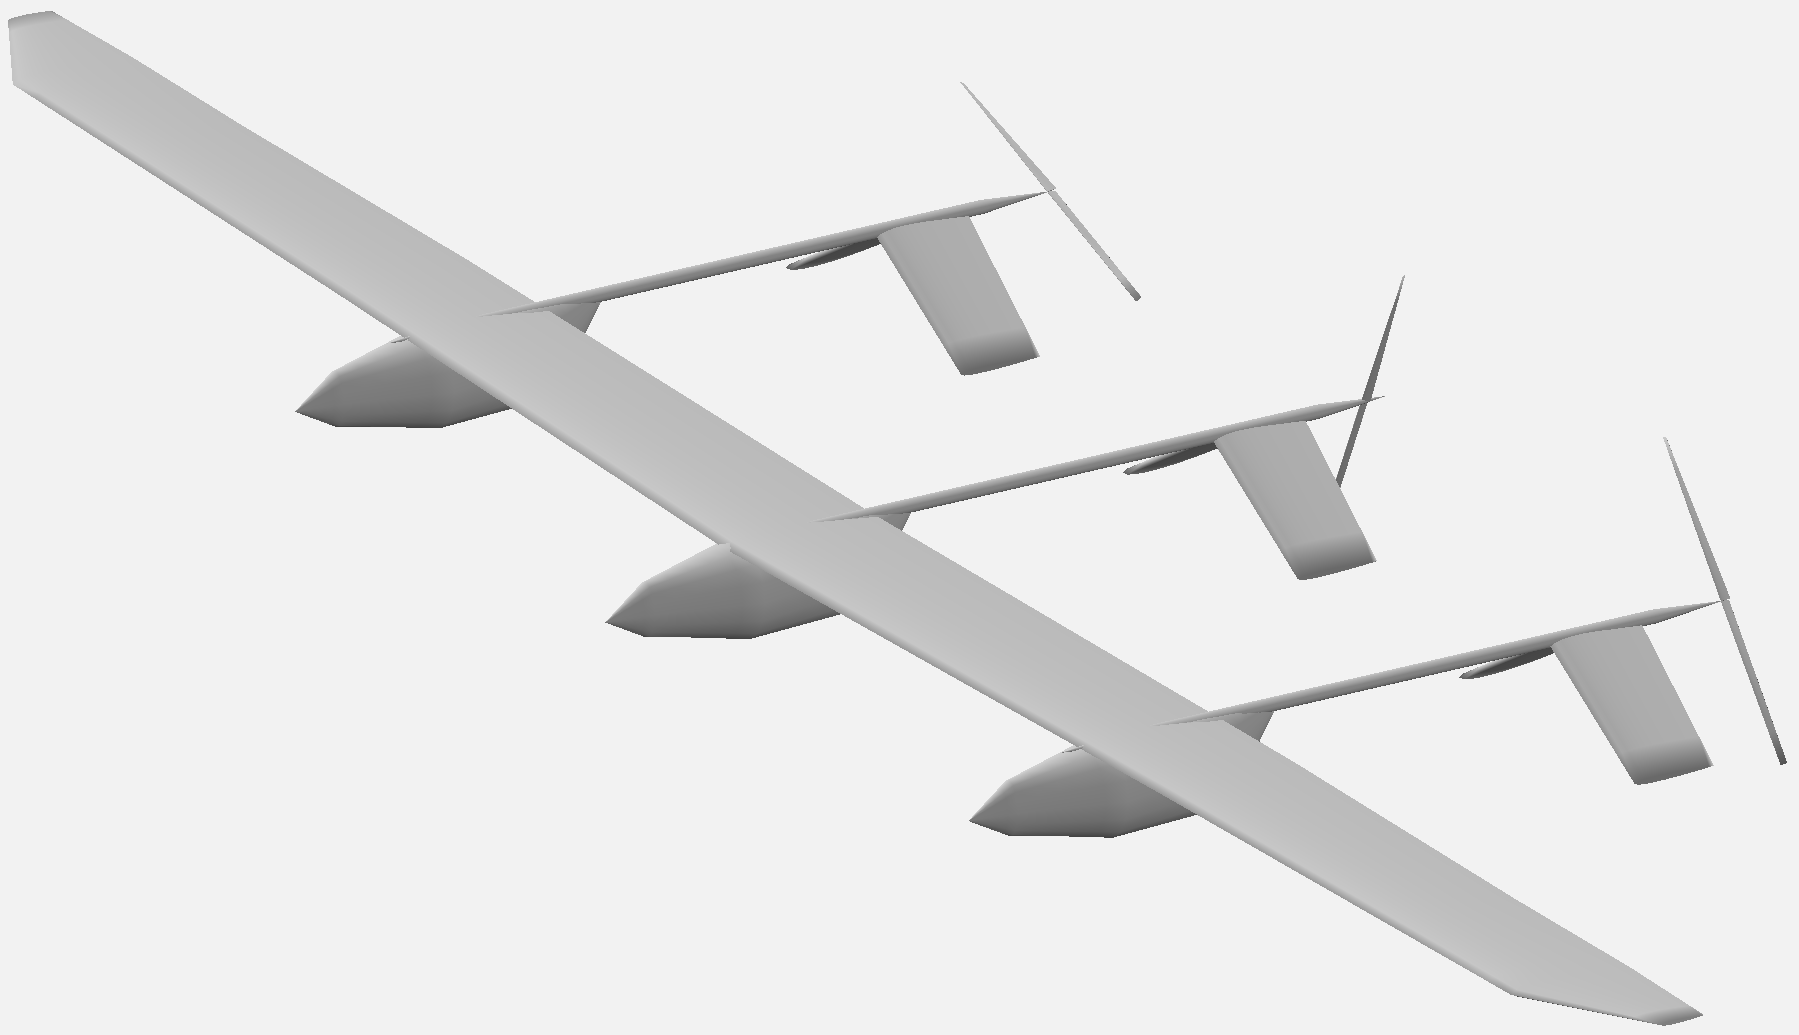
\includegraphics[width=\textwidth]{images/vsp_concept_solid}
    \end{figure}

  \section{Innovation}
    The nature of the highly flexible wing on this human powered aircraft will demand the use 
    of nonlinear structural models. A fully coupled high fidelity nonlinear structural, aerodynamic modeling method 
    will represent a significant advancement in the state­-of-­the-­art for aero­-structural design. By also including 
    propeller effects on the aerodynamics of the wing, we will be demonstrating an even larger degree of multidisciplinary 
    coupling. 

    In addition, the extremely low available power levels for human powered aircraft demand laminar flow over as much of 
    the aircraft as possible. Because of the large deformations, its important to maintain laminar flow in the 
    as-flown condition. By using the coupled aero-structural analysis we can take deformations into account in the design 
    of the airfoils. 

    Lastly, the integration of multidisciplinary design optimization into all phases of the aircraft design process represents
    a tremendous opportunity to learn how it can be best utilized. By combining MDO, testing, and actual flight into a single 
    we gain the opportunity to iterate not just on the design but also on the design process itself. The ability to adjust the 
    MDO methods to better suit the design process is a unique and highly valuable opportunity. 

  
\section{Intellectual Property Statement}
    \begin{itemize}
        \item All models will be open sourced
        \item All design will be made publicly available via a detailed design report
        \item All codes will be shared via GitHub
    \end{itemize}

\section{Virtual Meetings and Collaboration Plan}
    \begin{itemize}
        \item GitHub used to coordinate all codes and model 
        \item GoogleHangout or other VITS System for monthly meeting
        \item Two in person multi-day meetings
    \end{itemize}

\section{Milestones and Deliverables}
    \subsection{Milestones}
        \begin{itemize}
            \item geometry model for the aircraft, including structural model (Glenn/AeroVelo) 11/30/2014
            \item geometry model for the propeller (Glenn/AeroVelo) 11/30/2014
            \item FEM (TACS) Model of the wing (GATech) 
            \item Aerodynamic Model of the Wing (Stanford/Ames)
            \item Coupled Aero-Propulsive Analysis in OpenMDAO (Glenn/Stanford)
            \item Coupled Aero-Structural Analysis in OpenMDAO (Glenn/GATech/Stanford) 
            \item Coupled Aero-Structural Optimization in OpenMDAO (Glenn/GATech/Stanford)
            \item Conceptual Design for Marathon Airplane (Glenn/AeroVelo) 1/30/2015
            \item Detailed Design for Marathon Airplane (Glenn/AeroVelo) 9/30/2015
        \end{itemize}

    \subsection{Deliverables}
        \subsubsection{Year 1}
            \begin{itemize}
                \item Structural Test Articles (AeroVelo)
                \item Aerodynamic Test Articles (AerVelo)
                \item Aerodynamic Models (Stanford)
                \item Structural Models (GaTech)
                \item Final Report (All)
            \end{itemize}
        \subsubsection{Year 2}
            \begin{itemize}
                \item Additional Testing?? 
                \item Structural Dynamic Analyses?? 
                \item Flying Airplane??
            \end{itemize}

  \section{Resource Planning}
    \subsection{Test Facilities}
    \subsection{Supercomputing Resources}

  \appendix

  \section{Budget}
    Maximum available funds: 750k 
    \begin{itemize}
        \item 1 FTE Glenn - 150k 
        \item NASA Glenn WYE Support 60k 
        \item 1 FTE Ames - 150k 
        \item .25 FTE Armstrong - 40k
        \item Wind Tunnel and Structural Testing - 100k 
        \item Stanford - 125k 
        \item GATech - 125k
    \end{itemize}

  \section{Resumes \& Qualifications}


  \bibliography{references}

\end{document}